\chapter{Estado da arte}
\minitoc
\label{chap:Estadodaarte}
\vspace{0.5cm}

%%%%%%%%%%%%%%%%%%%%%%%%%%%%%%%%%%%%%%%%%%%%%%%%%%%%%%%%%%%%%%%%%%%%%%%%%%%%%%%%
% Objetivo:                        %
%%%%%%%%%%%%%%%%%%%%%%%%%%%%%%%%%%%%%%%%%%%%%%%%%%%%%%%%%%%%%%%%%%%%%%%%%%%%%%%%

  \lettrine{N}{este} capítulo mostraranse as diversas alternativas no mercado da 
xestión de competicións así como se fará unha análise do software libre neste campo e do 
proceso de estandarización que se busca con este proxecto.

\clearpage

  \section{Competidores no mercado}

    \subsection{Follas de cálculo}
    As follas de cálculo é o sistema utilizado por excelencia para xestionar competicións.
    
    Un sistema rudimentario pero funcional, algunas federacións combinan en certa medida 
follas de cálculo e bases de datos sinxelas para crear as táboas das 
clasificacións e dos resultados, utilizando funcións que permiten automatizar algunhas 
tarefas como por exemplo o cálculo da clasificación dos equipos en función dos 
seus resultados ao longo da competición.

    \begin{figure}[h!]
	  \begin{center}
	    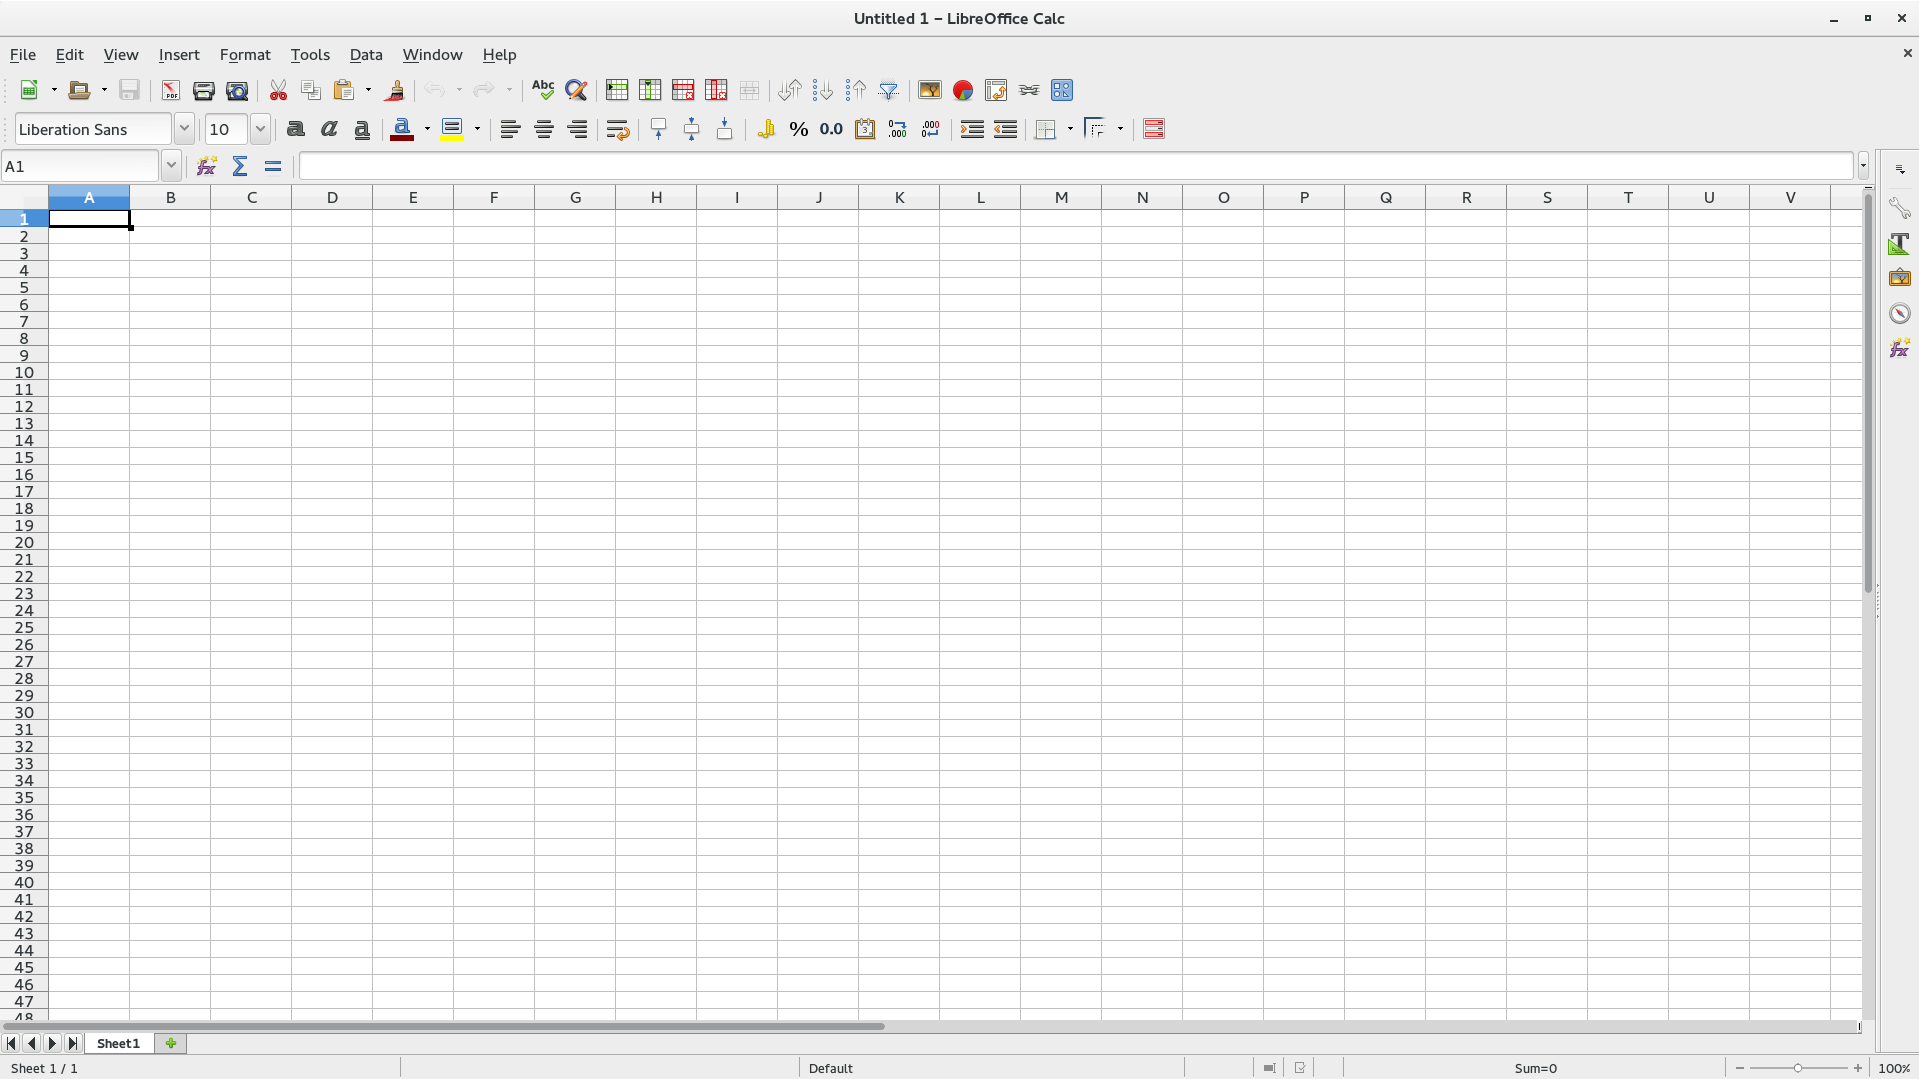
\includegraphics[width=0.8\textwidth]{./img/calculo.png}
	    \caption{Folla de cálculo}
	  \end{center}
    \end{figure}

    O sistema é moi versatil para usuarios experimentados pero implica un gran 
traballo manual e pode chegar a ser un suplicio para usuarios con poucos coñecementos de 
ofimática.

  As actas seguen a chegar en papel a federación e os datos deben ser introducidos nas 
diversas follas de cálculo (que en competicións de gran tamaño, vólvense inmanexables), 
revisando as sancións de xeito manual, polo que os erros na interpretación dos datos son 
habituáis.

\clearpage

    \subsection{Novanet}

      Novanet é unha empresa especializada na xestión de competicións de fútbol 
e o seu producto componse únicamente dunha aplicación web dende a que crear as 
clasificacións pero tamén modificar as actas dos partidos ou ver os resultados.

      No caso que nos incumbe, non dispón dunha aplicación que poida ser instalable nun 
teléfono móbil e os árbitros vense na obriga de acceder directamente a páxina web da 
federación para modificar as actas.
  
      Ademáis, non permite o funcionamento do sistema de forma offline xa que non foi 
pensado inicialmente para o caso, o que obriga a levar a acta en papel que se cubre 
igualmente a pesar de que logo o árbitro sube os datos a web cando chega a súa casa.

      A interfaz é bastante complexa, o cal é un problema xa que a meirande parte dos 
árbitros son de avanzada idade e polo tanto resúltalles dificil adaptarse.

      Por último mencionar que únicamente está pensada para funcionar en fútbol e fútbol 
sala.
	
      \begin{figure}[h!]
	\begin{center}
	  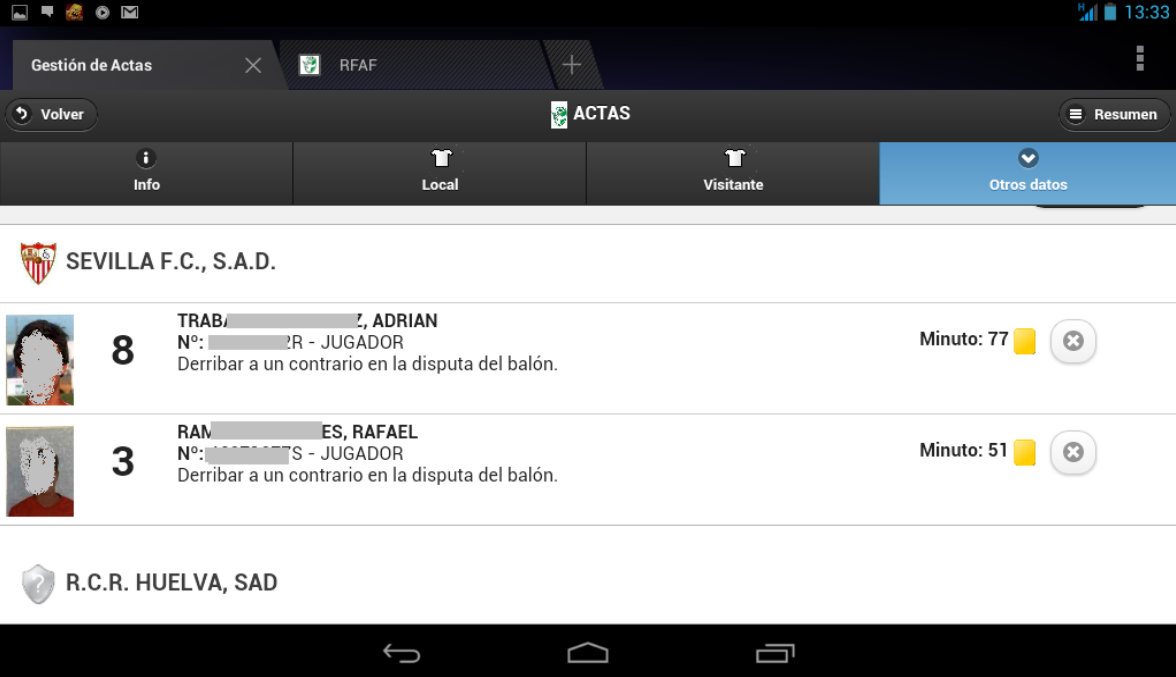
\includegraphics[width=0.8\textwidth]{./img/novanet-app.png}
	  \caption{Aplicación web de Novanet}
	\end{center}
      \end{figure}

\clearpage

    \subsection{Federatio}

    O caso de Federatio é moi similiar ao anterior xa que tampouco dispón dunha 
aplicación específica para a xestión de actas electrónicas de forma sinxela e polo tanto, 
os árbitros deben acceder a través da páxina web ao chegar a casa, para pasar os datos da 
acta física a versión electrónica.

    A interfaz dista de ser atractiva xa que apenas se renovou dende que comezou a 
funcionar entorno ao ano 2005 e non se atopa adaptada a móbiles, o que dificulta 
enormemente a labor dos árbitros.


      \begin{figure}[h!]
	\begin{center}
	  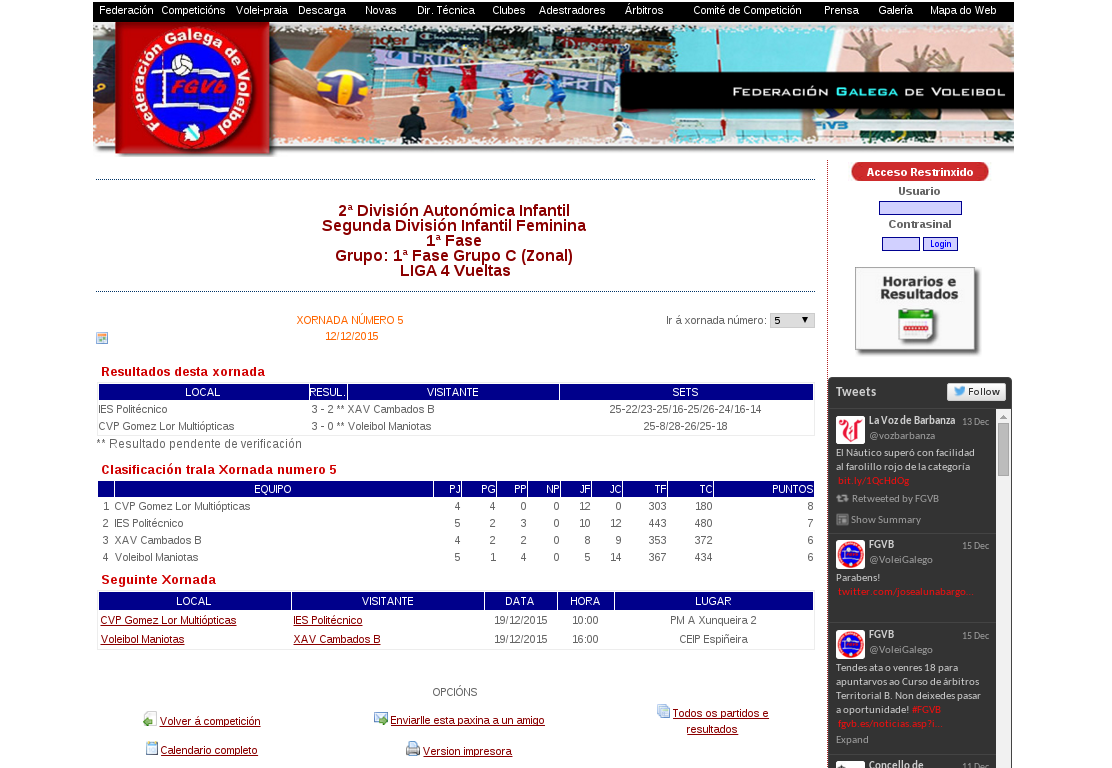
\includegraphics[width=0.8\textwidth]{./img/federatio-app.png}
	  \caption{Web da FGVB co sistema Federatio}
	\end{center}
      \end{figure}

\clearpage

    \subsection{miLeyenda}
  
    miLeyenda é unha plataforma de xestión de competicións na nube que permite 
aos administradores de federacións dispor tamén de unha aplicación móbil nativa 
para IOS e outra para Android.
    
    Dende esta aplicación poden xestionar gran parte dos parámetros das súas competicións 
entre os que se atopan as actas dos encontros.
  
    Así mesmo tamén dispoñen dunha aplicación para que os xogadores e clubes poidan ver 
os resultados e as clasificacións polo que o custe de mantemento das aplicacións elévase 
enormemente ao ter que soportar ata 4 apps móbiles diferentes.
    
    Esta é unha das grandes vantaxes de utilizar as tecnoloxías web que emprega VACmatch 
Mobile, permitíndo utilizar unha soá aplicación para calquera sistema operativo.

    A usabilidade das aplicacións é salientable e permite a xestión de diversos deportes 
pero a cambio non permite cubrir as actas de forma offline, un problema habitual ante a 
falta de cobertura nos diversos pavillóns e campos deportivos.
  
      \begin{figure}[h!]
	\begin{center}
	  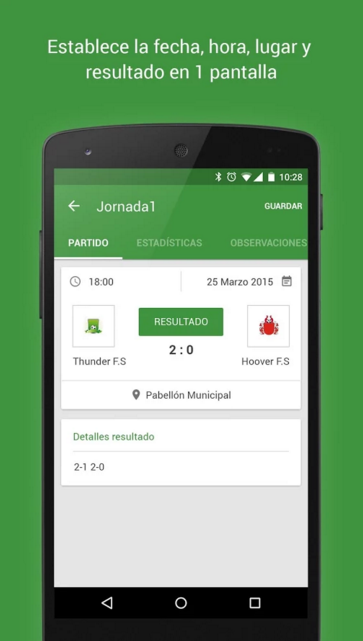
\includegraphics[width=0.3\textwidth]{./img/mileyenda-app.png}
	  \caption{APP móvil de MiLeyenda}
	\end{center}
      \end{figure}

\clearpage

    \subsection{Esportics}

    Esportics é unha startup española centrada na xestión de competicións 
deportivas e enfocada tremendamente cara o tenis e o paddel así como os deportes 
electrónicos.

A pesar de que a aplicación funciona para diversos deportes, a súa adaptación é bastante 
forzada en certos menús e a hora de estructurar as competicións.

    Únicamente dispón dunha páxina web adaptable a móbiles, aínda que a adaptación é 
mellorable, e polo tanto, non dispón dunha aplicación específica para que os árbitros 
poidan cubrir as actas de forma sinxela dende o seu teléfono.

    A usabilidade é aceptable pero mellorable, engadindo unha complexidade en certos 
menús que non son precisos e que provoca que os árbitros de avanzada idade, lles resulte 
tamén pouco intuitivo.

    \begin{figure}[h!]
      \begin{center}
	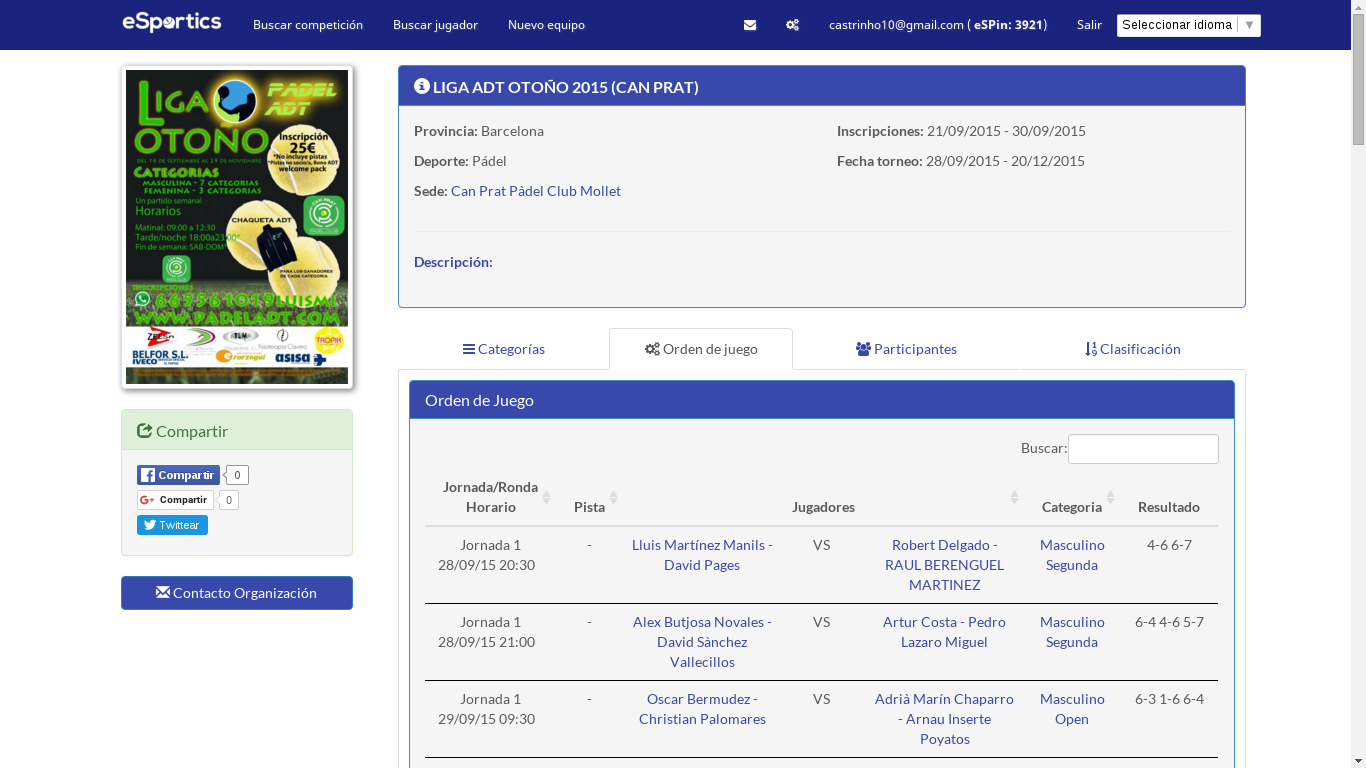
\includegraphics[width=\textwidth]{./img/esportics-app.png}
	\caption{Torneo de tenis na web de Esportics}
      \end{center}
    \end{figure}

\clearpage

    \subsection{Sportngin}

      \todo{citar desde o texto as figuras}
      
    Sportngin é unha solución integral para a xestión deportiva, probablemente un dos 
proxectos de referencia xa que dispón de aplicacións web e móbil para a xestión e a 
visualización de competicións.

    De feito, Sportngin permite a personalización da aplicación móbil a cada federación, 
cos seus logotipos, colores corporativos e incluso certos menús personalizables 
e incluso permite traballar de forma offline.
    
    A parte das funcións habituáis para xestionar as competicións e a creación de actas, 
con unha usabilidade moi coidada, aporta como valor engadido a visualización e xestión de 
noticias, fotos ou estadísticas da competición.

    Por último tamén permite aos entrenadores planificar adestramentos e incluso 
comunicarse cos seus xogadores a través da mensaxería interna.

    É sen dúbida o proxecto máis completo e a referencia a seguir.
 
    \begin{figure}[h!]
      \begin{center}
	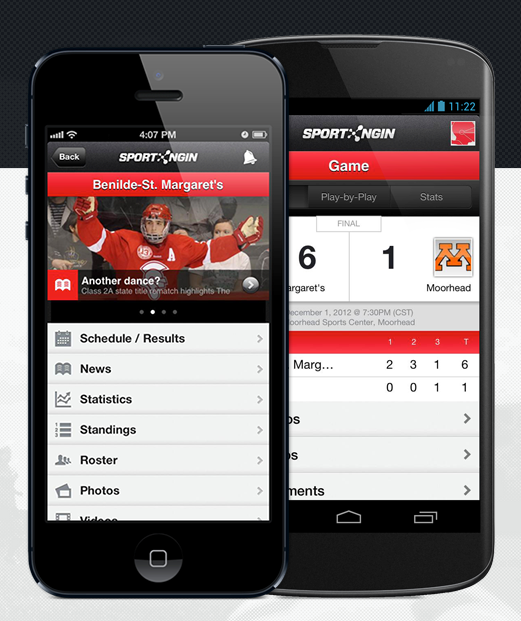
\includegraphics[width=0.5\textwidth]{./img/sportngin-app.png}
	\caption{APP móvil de Sportngin}
      \end{center}
    \end{figure}

\clearpage

    \subsection{Outras plataformas}
    Existen moitas ferramentas para a xestión de competicións e resultados pero apenas 
ningunha facilita aos árbitros unha plataforma sinxela e con unha usabilidade 
medianamente coidada.
    
    Tamén existen pequenas extensións coa idea de extender outras plataformas xenéricas 
para adaptalas a xestión de competicións como o \emph{Joomla! CMS sport extension} pero a 
función final é tremendamente limitada.
  
    Tamén temos outras propostas como \emph{Siguetuliga} que permite as persoas que 
se atopan vendo o partido, subir os resultados pero simplemente é un complemento, non 
facilita nin elimina o traballo dos xestores de competicións.

  \section{Aplicacións libres no mercado}
  
    O software libre é un sector en alza na actualidade, os proxectos colaborativos que 
forman o mundo \emph{Open Source} estanse a impor en múltiples mercados fronte as 
correspondentes alternativas privativas que adoitan a ser tremendamente costosas.

    Mesmo as grandes compañías TIC están a apostar por liberar parcial ou totalmente as 
súas tecnoloxías e productos, favorecendo un desenvolvemento colaborativo fronte a idea 
atrasada de secretismo e individualismo do modelo productivo habitual.

    Concretamente no mundo do deporte é tremendamente complicado atopar algún 
exemplo de aplicación baseada en software libre e as poucas existentes como 
\emph{zuluru} ou \emph{phpmysport} atópanse tremendamente atrasadas tanto en 
funcionalidades como no aspecto visual e por suposto sen ningún tipo de aplicación móbil 
para facilitar a xestión das actas polo que é importante propor unha alternativa 
ás aplicacións privativas habituais como é VACmatch Mobile.

  \section{Solución aberta e adaptable}
  Os xestores de competicións habitualmente realizan unha considerable inversión 
económica para que unha empresa de consultoría lles cree unha aplicación web ou de 
escritorio a medida para a súa xestión. Algunhas mesmo dispoñen de aplicacións móbiles 
para os árbitros pero que son específicas para dito sistema de xestión polo que a 
reutilización de aplicacións non é posible.

  Ademáis, estos sistemas son propietarios e o código non se atopa accesible 
polo que é imposible tratar de adaptar ditas aplicacións móbiles para outros 
sistemas de xestión.

  É por isto polo que se chegou a conclusión de que é preciso crear unha 
plataforma aberta como é VACmatch Mobile que porporciona unha aplicación 
software libre adaptable a diversos deportes e integra unha API de comunicacións 
aberta para a xestión de actas electrónicas e que permita a súa integración 
noutros sistemas de xestión entre os cales se atopa o sistema de VACmatch, unha 
implementación libre para a xestión de competicións.

  
